%
% ebene3punkte.tex
%
% (c) 2018 Prof Dr Andreas Müller, Hochschule Rapperswil
%
\documentclass[tikz,12pt]{standalone}
\usepackage{times}
\usepackage{amsmath}
\usepackage{txfonts}
\usepackage[utf8]{inputenc}
\usepackage{graphics}
\usetikzlibrary{arrows,intersections,math}
\usepackage{ifthen}
\begin{document}

\newboolean{showgrid}
\setboolean{showgrid}{false}
\def\breite{7}
\def\hoehe{4}

\begin{tikzpicture}[>=latex,thick]

% Povray Bild
\node at (0,0) {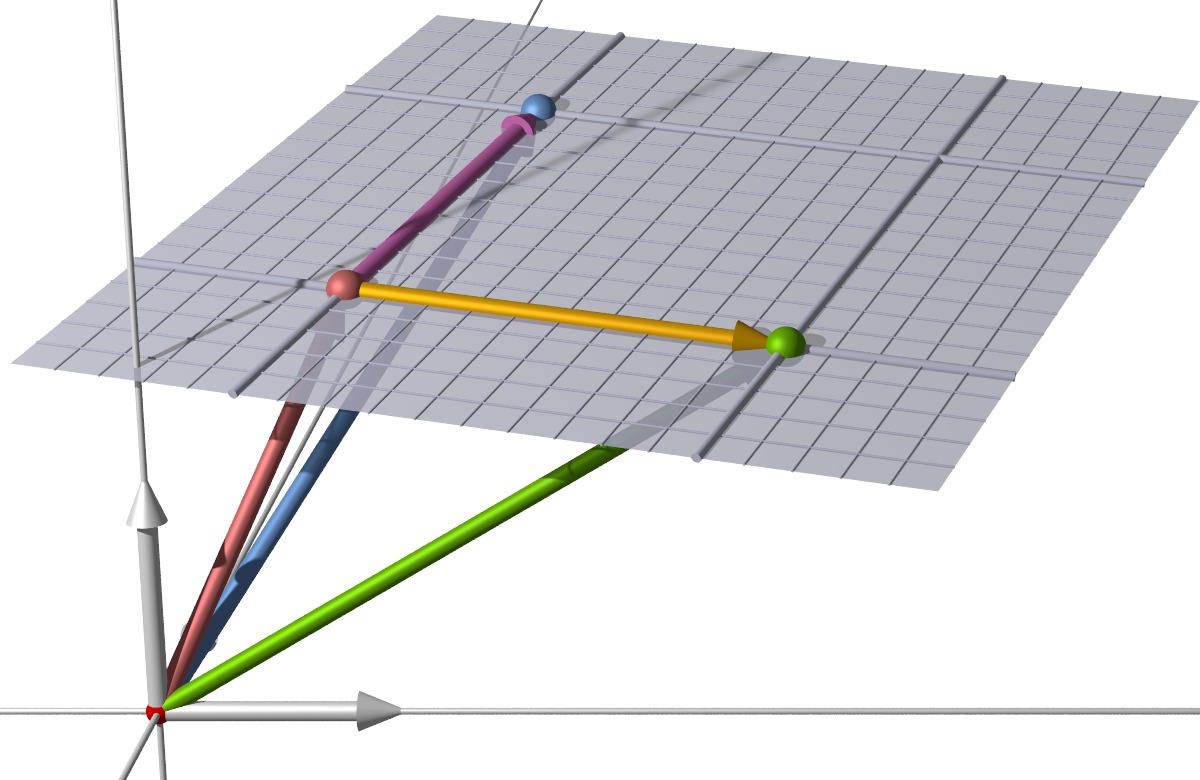
\includegraphics[width=14cm]{ebene3punkte.jpg}};

% Gitter
\ifthenelse{\boolean{showgrid}}{
\draw[step=0.1,line width=0.1pt] (-\breite,-\hoehe) grid (\breite, \hoehe);
\draw[step=0.5,line width=0.4pt] (-\breite,-\hoehe) grid (\breite, \hoehe);
\draw                            (-\breite,-\hoehe) grid (\breite, \hoehe);
\fill (0,0) circle[radius=0.05];
}{}

% Legende
\node at (-5.5,-3.5) {$O$};
\node at (-3.0,1.6) {$A$};
\node at (2.2,1.0) {$B$};
\node at (-0.7,3.7) {$C$};

\node at (-1,-1.5) [below] {$\vec{b}$};
\node at (-3,-1) {$\vec{c}$};
\node at (-4,-0.5) {$\vec{a}$};
\node at (0.8,0.8) [above] {$\vec{b}-\vec{a}$};
\node at (-1.5,2.7) [above left] {$\vec{c}-\vec{a}$};

\node at (-2.5,-3.6) [above] {$\vec{e}_1$};
\node at (-5.5,-1.4) [left] {$\vec{e}_3$};

\node at (5.5,3.0) {$\sigma$};

\end{tikzpicture}

\end{document}

